
\section{Erweiterung}
Für die Erweiterung wird der Microsoft Academic Knowledge Graph benutzt. Da wir hier nur suchen und einzelne Publikationen nur extrahieren müssen lohnt sich die Vorgehensweise mit Dumpfiles nicht. Da sie dazu auch noch mehrfach so groß wären. Deswegen verwenden wir hier das Project Academic Knowledge. In diesem Projekt gibt es die Academic Search API. Also eine Schnittstelle mit der man in dem Graph suchen und Daten auslesen kann. Es werden 4 verschiedene REST API's zur Verfügung gestellt. CalcHistogram, Evaluate, Similarity und Interpret. 

Der erste ist CalcHistogram hier werden alle such Ergebnisse zusammen gerechnet und ein Histogramm darüber erstellt. Also man erhält eine Häufigkeitsverteilung. Der zweite ist Evaluate diese Anfrage wird benutzt um seine Eingabe automatisch zu vervollständigen. Der Dritte ist Similarity hier werden 2 Texte auf Gemeinsamkeiten überprüft. In dem Fall wird Evaluate verwendet da wir weder ein Histogramm oder noch einen Vergleich brauchen. Mit Evaluate können normale Suchanfragen gestellt werden und es wird eine Menge von Entitäten zurückgegeben die dazu passen. Für unseren Fall suchen wir nach dem Titel. Hier lässt sich die Rückgabe auf bestimmte Attribute verringern. Wir brauchen nur die zitierten Publikationen. Deshalb beschränken wir die Ausgabeattribute auf 'CitCon'. Dies gibt uns die Id und den Abschnitt der Zitiert wurde. Da der zitierte Abschnitt immer mit übergeben wird fügen wir ihn mit in die Datenbank ein. Nun müssen wir die Id nur noch in einen Titel umwandeln um ihn mit unserer Datenbank in Verbindung zubringen. Dazu beschränken wir die Attribute auf 'Ti' um nur die Titel zu erhalten. Diesen Titel finden wir nun in der Datenbank und verbinden ihn mit der Publikation die ihn zitiert.

\begin{figure}[!htb]
	\centering
	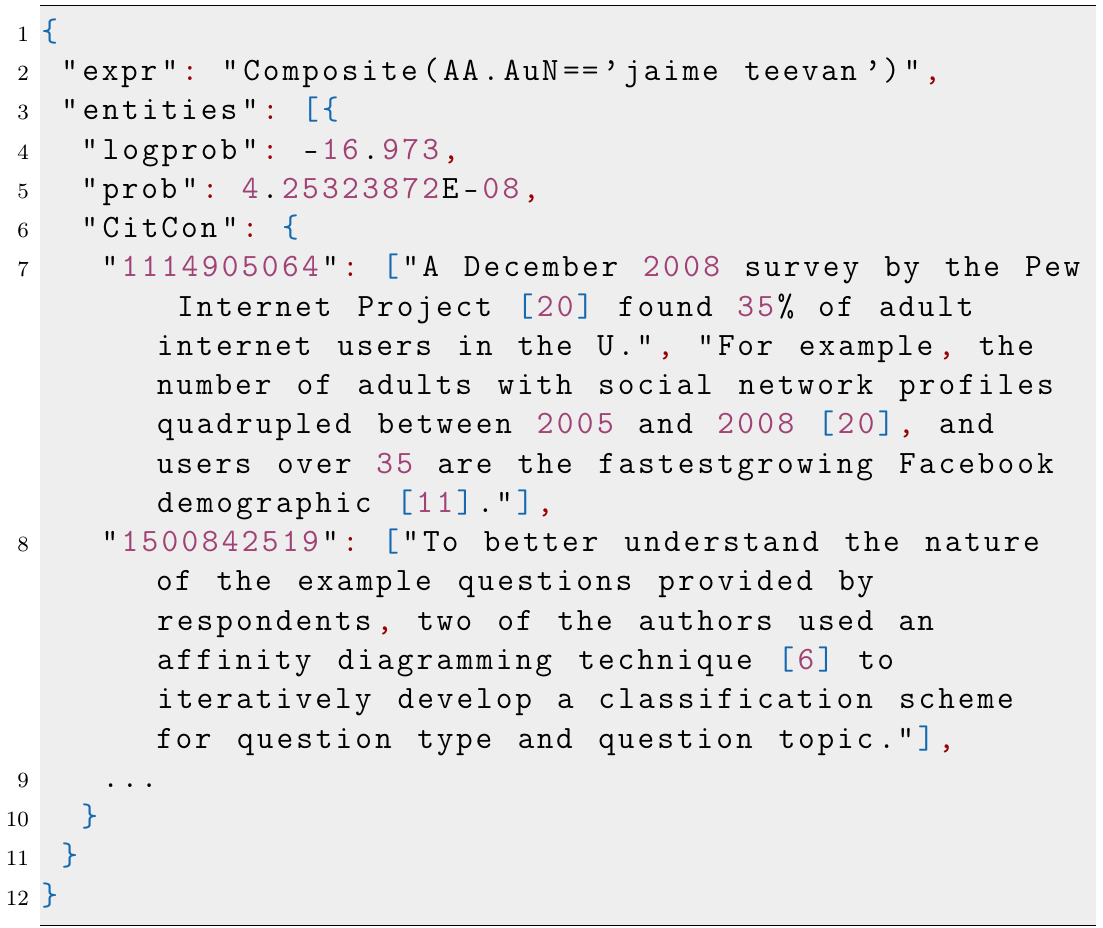
\includegraphics[width=12cm,keepaspectratio]{bilder/ResponseBeispiel}
	\caption{Response Beispiel}
	\label{fig:response-beispiel}
\end{figure}

Diese Response ist im JSON-Format. Diese dient genau wie XML für die Speicherung von menschlich lesbaren Daten. Der hier gezeigte Ausdruck ist nur ein Beispiel. Denn in der Expression wird ein Autor gesucht und nicht nach einem Titel. Da die Responses sehr kurz sein werden, müssen wir keinen Parser selber schreiben. Somit können wir einen fertigen Parser benutzen der uns die Daten raus filtert. Nun müssen wir nur die 2 Anfragen senden .

Mit der API kommt aber auch an eine Grenze. Im Monat dürfen nur 10.000 Transaktionen getätigt werden. Dadurch werden hier nur selektive Beispiele präsentiert. Deshalb haben wir eine Funktion die die ersten 100 Publikationen aus gibt. Mit diesen 100 werden wir die Zitate Testen und begutachten.